
%% See poetry_questions_full.tex for a four-column version


\begin{table}[t]
{\small
\def\arraystretch{1.1}
\begin{tabular}{p{1.8in}p{1in}}
\textbf{Question} & \textbf{Agent concerned} \\[.1cm]
\textbf{\emph{Word level}} & \\
What is are dictionary definitions of this word? & WordNet expert \\
What are its etymological roots? & Etymology expert \\
%%%%%%%%%%%%%%%%%%%%%%%%%%%%%%%%%%%%%%%%%%%%%%%%%%%%%%%%%%%%%%%%%%%%%%%%%%%%%%%%
Where did this word come from? & Provenance expert \\
What pronouns are used in the poem? & Pronoun expert\\[.2cm]
%%%%%%%%%%%%%%%%%%%%%%%%%%%%%%%%%%%%%%%%%%%%%%%%%%%%%%%%%%%%%%%%%%%%%%%%%%%%%%%%
\textbf{\emph{Phrase level}} & \\
What are the components? & Keywords expert \\
Do the components have a negative or positive connotation? & Association expert \\
What are the modifiers attached to the components? & Modifer expert \\[.5cm]
%%%
\textbf{\emph{Sentence level}} & \\
What is the parse tree? & Grammar expert \\[.2cm]
%%%%%%%%%%%%%%%%%%%%%%%%%%%%%%%%%%%%%%%%%%%%%%%%%%%%%%%%%%%%%%%%%%%%%%%%%%%%%%%%
\textbf{\emph{Line level}} & \\
How long is the line? & Counting expert \\
Where does it break? & Breathing expert \\
Where is there white space? & Position expert\\[.2cm]
%%%%%%%%%%%%%%%%%%%%%%%%%%%%%%%%%%%%%%%%%%%%%%%%%%%%%%%%%%%%%%%%%%%%%%%%%%%%%%%%
\textbf{\emph{Poem level}} & \\
How are terms that exhibit emotion distributed within the poem? & Distribution expert\\
Where is there alliteration (rhyme, consonance) in the poem? & Phonics expert \\
Does the poem have a metrical structure? & Rhythm expert \\
How repetitive is the poem? & Repetition expert \\
Does the poem cohere? & Thematic expert \\
Does the poem have a progression? & Narrative expert \\
Where are the various elements of the poem concentrated? & Entropy expert 
\end{tabular}
}
\caption{Questions we imagine a computer would currently be capable of answering when reading a poem\label{tab:questions_for_computational_agents}}
\end{table}

\section{Bridges between `theory' and `practice'}

Our \emph{ansatz} is that the Workshop could serve as a way to develop a process-based theory of poetics.
There are certain prerequisites.  In addition to the presentation of
written work, an underlying context, shared
(with respect to differing points of view) by the poet and the reader/listener
(see Figure \ref{fig:cycles}).  Participants are assumed to
have relatively stable, enduring but evolving, identities -- either might be able to ask
``Who am \emph{I}?''  and ``Who are \emph{you}?'' \cite[p. 251]{bakhtin1984problems}. 
Answers would acknowledge a prepared mind with certain prior questions, abilities, involvements, and so on.
However, in the Workshop, the discussion focuses solely on the work itself.
The Workshop provides an objective space in which the poet and readers can observe and
participate in the creative process.

Table \ref{tab:questions_for_human_readers} contains a list of questions that a reasonably
sophisticated poetry reader might ask about poems.  This is complemented by a list of
questions that could be addressed, in a straightforward programmatic manner (Table \ref{tab:questions_for_computational_agents}).  
Each of the examples listed in the right-hand column of Table \ref{tab:questions_for_human_readers} (and a plethora
that are not listed) present a way of thinking about the poem.  We can see these as roughly analogous to the agents in Table \ref{tab:questions_for_computational_agents} \cite{minsky2006emotion}.

To begin, in response to a computer-generated poem:

{\itshape
\begin{verse}
%Demon dog\\[\baselineskip]
%
Oh dog the mysterious demon\\
Why do you feel startle of attention?\\
Oh demon the lonely encounter\\
ghostly elusive ruler\\
Oh encounter the horrible glimpse\\
helpless introspective consciousness\\
\end{verse}
}

A human critic might offer the following feedback:

\begin{quotation}
~\vspace{-1\baselineskip}
\begin{enumerate}
\item The use of the word \emph{mysterious} in the first line has no
  resolution, real or attempted, or quest to find one.
%
\item The use of the word \emph{attention} is not being interrogated
  or acknowledged for its importance.  Its qualifying word is
  \emph{startle}, used here as an adjective; acknowledging the fact
  that the attention is noted, but is not yet part of the transformative
  of the poem.
%
\item This is repeated in the next references to the aesthetic
  experience as a \emph{lonely encounter}, \emph{exclusive
    ruler}, \emph{horrible glimpse} and \emph{introspective consciousness}.
%
\item The contact made between the poem and its own
  construction is qualified in negative terms attached to the words
  \emph{demon}, \emph{encounter} and \emph{consciousness}.
%
\item This poem does not welcome the intimacy of bringing anything to
  aesthetic consciousness so that it might be expressed. Why do I say
  that? Because the words are generalised and \emph{horribly}
  imprecise.
%
\item  The poem does not move toward a better understanding of the ideas it alludes to.
  The vocabulary seems to associate exploration with fear and isolation and this is
  (paradoxically) quite an interesting acknowledgment of the poem’s
  refusal to go anywhere i.e.~to become a thing transformed by a creative
  process.
\end{enumerate}
\end{quotation}

Each of these six points is \emph{dual-voiced} in the sense that the
critic is relaying the words of the poem with a new emphasis.  Each such
statement is one side of a micro-dialogue
\cite[p. 73]{bakhtin1984problems}.  The challenge is, of course, to
bring the observations into the awareness of the computer poet, across
the ``analogue divide.''
%
Care should be taken not just to blythely program the computer with more rules, but
rather to give attention to facilitating the process of learning new rules contextually.
We continue with the example from this point of view in the following section.

First we will consider a reversal of roles, with the
computer in the position of critic, looking at a passage from an
historical piece of poetry.  We have selected a passage from Robert Burns that might have --
but in fact did not -- serve as a model for the poem generated above.

{\itshape
\begin{verse}
I'm truly sorry man's dominion\\
Has broken Nature's social union,\\
An' justifies that ill opinion\\
Which makes thee startle\\
At me, thy poor, earth born companion\\
An' fellow mortal!\\
\end{verse}
}

Naturally, the first problem is for the computer to \emph{read} the
poem.  One of
the approaches that is most appealing from our point of view is the
automatic generation of a semantic network from the input text
\cite{harrington2007asknet}.  We could straightforwardly extend the methods of Harrington
and Clark with notions drawn from Table
\ref{tab:questions_for_computational_agents}.

\begin{quotation}
~\vspace{-1\baselineskip}
\begin{enumerate}
\item begins with \emph{I}/\emph{me}, locating the \emph{poor, earth born} poet
\item \emph{thee}/\emph{thy} is another person, possibly the reader, who becomes \emph{startled}
\item singular \emph{I} contrasts with the class \emph{man}
\item \emph{sorry} is a sad emotion
\item \emph{truly} exaggerates sorry
\item \emph{dominion} is large
\item \emph{broken} and \emph{union} are opposites
\item \emph{sorry} and \emph{justifies} are opposites
\item \emph{union}, \emph{companion}, and \emph{fellow} are positive words about relationship and joining
\item \emph{broken}, \emph{ill}, \emph{poor}, \emph{startle} and \emph{mortal} are related to frailty
\item \emph{born} and \emph{mortal} are related
\item There are a lot of rhymes in the poem, at the end of the lines, enjambed.
\end{enumerate}
\end{quotation}
These comments are very different from the other reading above, and are differently interesting.

We've demonstrated that the computer is capable of asking objective questions of a poem.  A similar semantic network approach would allow it to listen to feedback and take it on board, even when it doesn't understand the ways of thinking that generate this feedback.  Again, this links the process of reading and writing poetry to a process of dialogue.

\section{Seeds for a FloWr Garden}

\begin{figure}[t]
\begin{center}
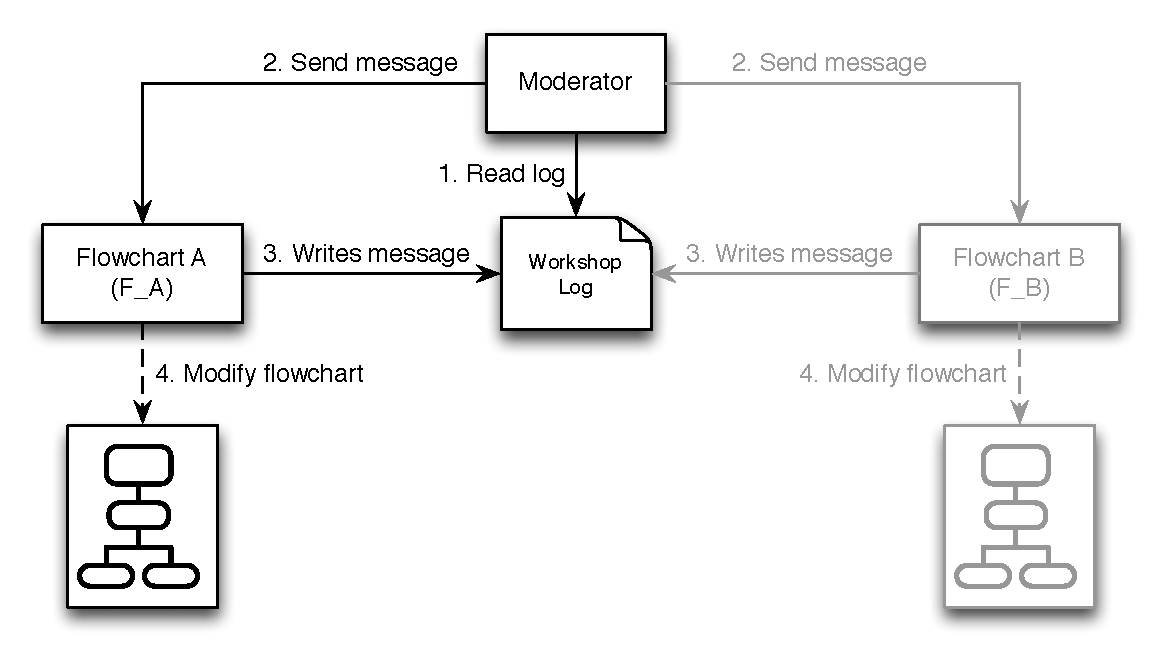
\includegraphics[width=\columnwidth]{figures/Schema}
\end{center}
\caption{Schematic diagram for a workshop built in the FloWr system\label{fig:workshop_schematic}}
\end{figure}

Keeping in mind the current limitations of FloWr -- no looping or conditionals, only running one flowchart at a time and in one direction -- a {\em conversation} between ProcessNodes or flowcharts is not immediately feasible.  Figure \ref{fig:workshop_schematic} represents a hypothetical design in which a Workshop could take place with a minimally-altered version of FloWr. As shown in Figure \ref{fig:workshop_schematic}, each participant in the Workshop would be represented by a single node. One of these nodes is a {\em moderator} in charge of dictating the interaction between the participants of the Workshop, while the rest represent {\em flowcharts} that have the ability to modify their own connections according to the discussions from the Workshop -- this can be achieved by exploiting the scripting mechanism of FloWr and dynamically loading the new structure of the flowchart. Moreover, a shared \emph{log} would contain the history of the messages exchanged during the Workshop and a queue of messages waiting to be delivered. We define four different types of messages that can be exchanged:
\begin{itemize}
% \item {\bf\em advertisement} of the overall capabilities of a participant.
\item {\bf\em comments} about specific elements of a poem, or more general appreciations of it.
\item {\bf\em questions} about specific details of a participant's capabilities; for instance, the questions can vary from simple requests of sources of information (e.g. files, input from another node, which resources a flowchart uses, etc.) to process-specific details (e.g. current conditions, purpose, other outstanding questions, etc.)
\item {\bf\em answers} would be associated to previous questions and may contain simple text such as an url for the source of information, or a piece of script representing a node used by a flowchart.
\item {\bf\em suggestions} are changes proposed by one participant to another. Similar to the answer, this can be as simple as suggesting the change of an information source, or more complex as suggesting the replacement of a node for an alternative node.
\end{itemize}

A Workshop session follows this communication protocol:
\begin{enumerate}
\item The moderator initialises an empty log and sends a message to the flowcharts to indicate that the session has started. 
\item The flowcharts start writing messages in the log.
\item The moderator checks the current state of the workshop by reading the log. \label{step:loop}
\item The moderator selects the next message in the queue and pass it to the target flowchart. 
\item The flowchart reads the message and acts accordingly by either (i) modifying its connections or (ii) sending a message back; i.e. writes in the log. 
\item Step \ref{step:loop} is repeated until no further message are left in the queue.
\end{enumerate}

% This protocol rises the following questions: from the suggestions received (i) which one is the best option?  (ii) how many options do we listen to before we even try to make a decision?   

\paragraph{Example.}
Figure \ref{poetryGeneratorFlowchart} shows the poetry generator flowchart that generates the poem about the ``demon dog'' presented above. The flowchart uses two linguistic resources: ConceptNet \cite{ConceptNet}, a semantic network of common knowledge, and Disco \cite{Disco}, a semantic similarity words retrieval system. Let us assume the human critic $\mathbf{A}$ has access to the system through a ``UI flowchart'' like a Read-Eval-Print Loop (REPL), and the poetry generator $\mathbf{B}$ is mainly concerned with maintaining a generative flowchart like the one shown in the figure. The following exchange of messages can occur:

\begin{enumerate}
\item \textbf{Comment from participant $\mathbf{A}$ to participant $\mathbf{B}$}: {\em The words ``lonely encounter'' and ``elusive ruler'' in lines 2 and 3 are generalised and imprecise}.
\item \textbf{Question from participant $\mathbf{B}$ to participant $\mathbf{A}$}: {\em I identify the processes {\em Disco3} and {\em Disco4} as the source of the problem. Can you suggest an alternative to Disco?} 
\item \textbf{Suggestions from participant $\mathbf{A}$ to participant $\mathbf{B}$}: {\em Use WordNet or the Historical Thesaurus to find more expressive and specific terms for the core concepts in the poem; try to link the core concepts together by chaining together related concepts in ConceptNet or WordNet.}%\footnote{\url{http://wordnet.princeton.edu/}}\textsuperscript{,}\footnote{\url{http://historicalthesaurus.arts.gla.ac.uk/}}
\item \textbf{Action executed by participant $\mathbf{B}$}: Receives suggestions, creates several alternative versions of the script, executes them and decides which one is most coherent and which conveys a sense of narrative.
\end{enumerate}

\noindent From this exchange, the computer might learn (without ever being explicitly told) that expressive terms and narratives are related, and it might find a way to produce coherent poems with a narrative structure.

\paragraph{Remark.}
Since the computer has source code instead of a brain, we can use it to do control studies with process.  However, in general source code does not completely determine process: contextual effects are what make an experiment an experiment.  As described in \cite{cook2013mechanics}, code does often include hints about context.  This is related to our theme of embedding process within an artefact.
%
In this connection, one extension to FloWr that would help to facilitate dialogue between flowcharts would be to add machine-readable \emph{commentary} to ProcessNodes.  Commentaries would label a node's inputs and outputs, describe its basic purpose, and providing information about procedure, conditional behaviour, mappings between processes and elements of the poem (like the mapping between Disco3 and ``lonely encounter''). 
% This would enable basic procedural communication between flowcharts and would also allow the system to identify where to apply suggestions for new versions of a flowchart as suggested in a workshop session. 

\begin{figure}[t]
\begin{center}
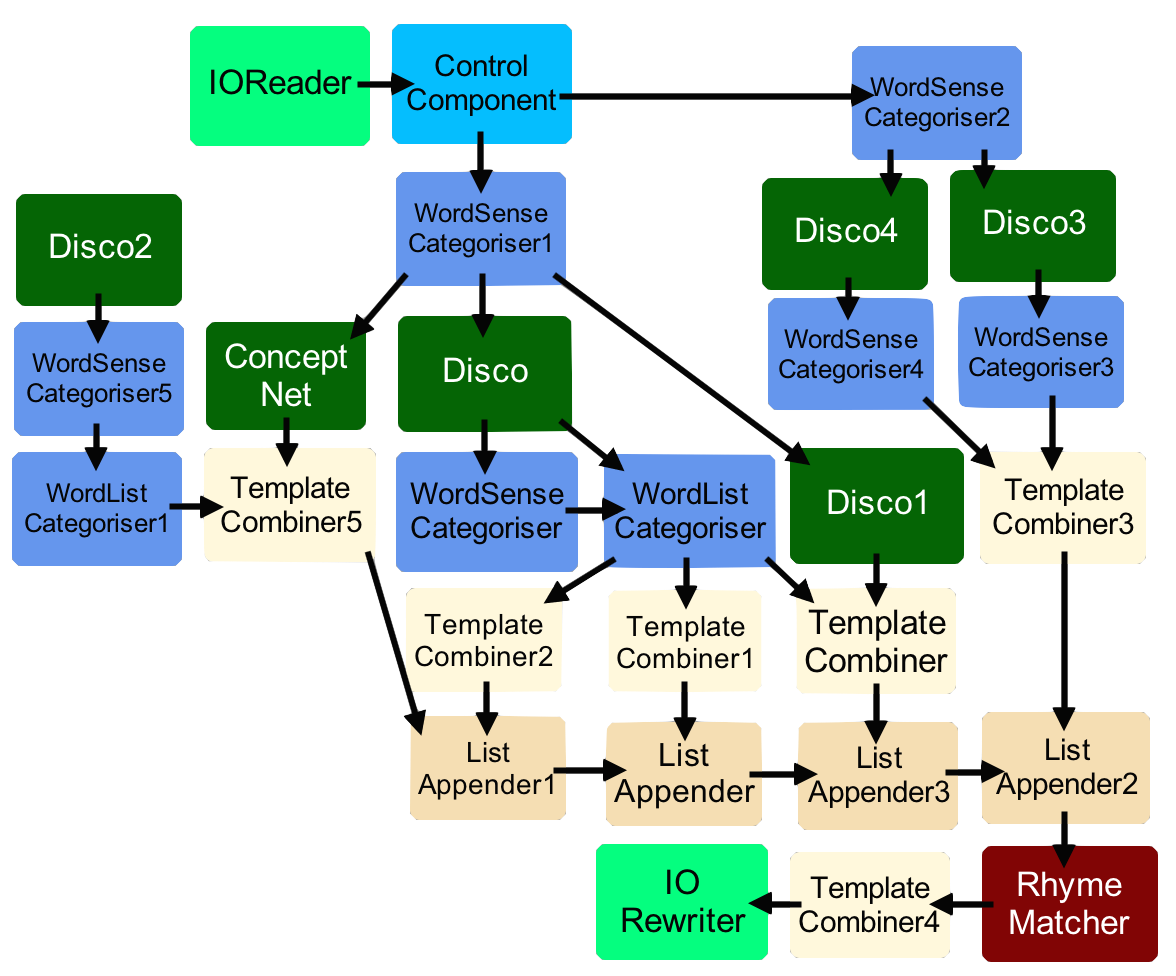
\includegraphics[width=\columnwidth]{./figures/PoemsFlowchart.png}
\caption{The flowchart that generated the ``demon dog'' poem}
\label{poetryGeneratorFlowchart}
\end{center}
\end{figure}

\paragraph{Down the garden path?}
Altered versions of a flowchart \cite{charnley2014flowr} can be seen as parallel solutions that could be executed and compared on a population basis with respect to some pre-specified metrics in order to make an informed decision on which suggestion(s) to follow, as hinted in the last step of the example.  In \cite{colton-assessingprogress} we explored the related idea of modelling system progress over time.  Learning new rules contextually would offer one clear measure of progress.  While these features sound good, we caution the reader that FloWr is still a research prototype, and considerable work would be required to realise the ideas we've described in FloWr or any other platform we're aware of.

%%% Local Variables: 
%%% mode: latex
%%% TeX-master: "mathsICCC"
%%% End: 
